%06.06-13.06
%3. Design => ca. 15 Seiten
%- Optimierungs/Wissenszyklus Abstrakt
%- Leistungs-Vorhersage (Predictor)
%- Reduktion von Werten zu Klassen => Preprocessing
%- Ursachen-Klassifikator (Cached vs. Uncached mit Labels die von
%Benutzern zu definieren sind). Beispielgraph einfach von Daten
%übernehmen.
%- Extraction von Wissen aus Decision Trees => verweis nach hinten.
%- Einsatz von Decision Tree (parameterisierung) ??? Sonst Implementierung.
%- Beispielhafte Ausgabe eines Programlaufs
%=> Bei Terminierung des Programs wollen wir ja sehen, dass der die
%Gründe und Bewertung vornimmt. Wieviel I/O In Klasse 1, 2....
%(Entsprechend der Namen).

\newpage

\section{Design}
Das Design des Programms soll darauf ausgerichtet werden, um uns den 
\textit{Optimierung/Wissenszyklus, Leistungsprädiktor, Ursachen-Klassifikator, Wissensextraktion, Ausgabe des Plugins}

\subsection{Optimierungs/Wissenszyklus Abstrakt}

Die E/A-Operationen werden vom Intrumentierer abgefangen, in die Aktivitäten umgewandelt und in einer Spurdatei gespeichert.
Nach der Ausführung der Anwendung beinhaltet die Spurdatei eine Datensammlung, die von einer Analysesoftware verarbeitet werden kann.
Die Analysesoftware lernt von den Daten und erstellt ein Modell, die Leistungswerte vorhersagen kann.
Der Optimierer nutzt dieses Modell, um optimale Parameter zu bestimmen und der Anwendung zur Verfügung zu stellen.
Die Anwendung nutzt diese Parameter für die E/A-Operationen.


\begin{figure}[ht]
	\centering
	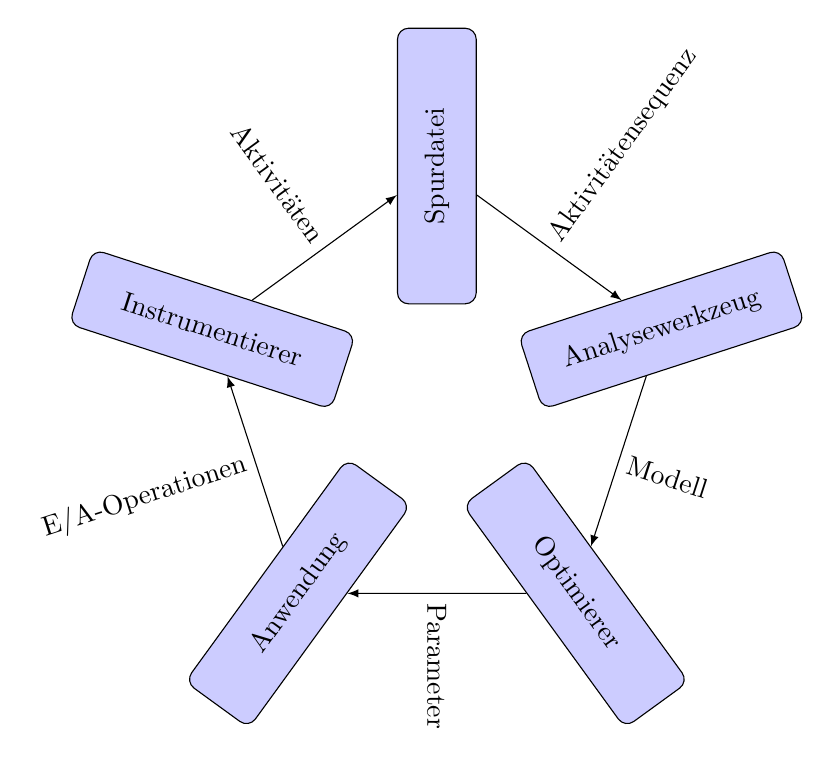
\begin{tikzpicture}
	[
		remember picture,
		>=latex reversed,
		phase/.style={draw,rounded corners, fill=blue!20, align=center, minimum height=1cm, minimum width=3.5cm},
		node distance=5mm and 5mm
	]

	\def\dist{3cm}

	\coordinate
	[]
		(center) at (0,0);

		\path (0,0) (90:\dist) node
		[phase, rotate=90, label={[align=center]270:{}}]
		(phase00)
		{Spurdatei};

		\path (0,0) (18:\dist) node
		[phase, rotate=18, label={[align=center]270:{}}]
		(phase01)
		{Analysewerkzeug};

		\path (0,0) (-54:\dist) node
		[phase, rotate=-54, label={[align=center]270:{}}]
		(phase02)
		{Optimierer};

		\path (0,0) (234:\dist) node
		[phase, rotate=54, label={[align=center]270:{}}]
		(phase03)
		{Anwendung};

		\path (0,0) (162:\dist) node
		[phase, rotate=-18, label={[align=center]90:{}}]
		(phase04)
		{Instrumentierer};

		\path
		[->, >=latex]
		(phase00)       edge node[rotate=54, right] (sequenz) {Aktivitätensequenz}    (phase01)
		(phase01)       edge node[rotate=-18, right] (model) {Modell}   (phase02)
		(phase02)       edge node[rotate=-90, right] (params) {Parameter}    (phase03)
		(phase03)       edge node[rotate=18, left] (ops) {E/A-Operationen}(phase04)
		(phase04)       edge node[rotate=-54, left] (act) {Aktivitäten}   (phase00);


\end{tikzpicture}

	\label{fig:des:opt_cycle}
	\caption{Optimierungs- / Wissenszyklus}
\end{figure}

In dieser Arbeit wird allerding nicht der gesamte Zyklus bearbeitet.
Dieser Zyklus setzt voraus, dass die Anwendung die optimalen Parameter nutzen kann. 
Solche Anwendungen gibt es nocht.
Die ersten theoretischen Ansätze für einen Optimierer wurde bereits in der Arbeit \todo{Referenz} behandelt und kann in den Zyklus leicht integriert werden.

\subsection{Leistungsprädiktor}
Die in der Arbeit verwendete Lehrnverfahren unterstützen keine Fortsetzung der Trainingsphase.
D.h. es müssen erst die Trainingsdaten gesammelt werden und dann kann das Modell trainiert werden.
Fertige Modelle können nachträglich mit weiteren Daten nicht verbessert werden.
Diese Eigenschaft der Lernverfahren spiegelt sich direkt in der Funktionsweise des Plugins. 
In der ersten Phase \figref{fig:des:perf_training} erzeugt das Plugin aus der Aktivitätensequenz Trainingsdaten, trainiert damit die Modelle und speichert sie in einer Datei ab.
In der zweiten Phase erzeugt das Plugin aus der Aktivitätensequenz eine Testmenge und wendet sie an.

\begin{figure}[ht]
	\hfill
	\subfigure[Training]{
		\begin{tikzpicture}
	[
		%remember picture,
		>=latex reversed,
		node distance=5mm and 5mm,
		flowchart
	]

	\node
		[block]
		(start)
		{Start};
	\node
		[block, below=of start]
		(get)
		{nehme Aktivität};
	\node
		[block,below=of get]
		(compute)
		{erzeuge Beispiel};
	\node
		[block,below=of compute]
		(save)
		{füge zu Trainingsdaten hinzu};
	\node
		[decision, below=of save]
		(decide)
		{Sequenzende?};
	\node
		[block,below=of decide]
		(train)
		{trainiere Modell};
	\node
		[block, below=of train]
		(results)
		{speichere Modell};
	\node
		[block, below=of results]
		(end)
		{Ende};

	\path
		[->, >=latex]
		(start) edge (get)
		(get) edge (compute)
		(compute) edge (save)
		(save) edge (decide)
		(decide) edge node[near start, right] {ja} (train) 
		(train) edge (results)
		(results) edge (end);
	
	\path
		[line]
		(decide) edge [out=180, in=180] node[near start, left] {nein}  (get);

\end{tikzpicture}


		\label{fig:des:perf_training}
	}
	\hfill
	\subfigure[Vorhersage]{
		\begin{tikzpicture}
	[
		%remember picture,
		>=latex reversed,
		node distance=5mm and 5mm,
		flowchart
	]

	\node
		[block]
		(start)
		{Start};
	\node
		[block, below=of start]
		(load)
		{lade Modell};
	\node
		[block,below=of load]
		(get)
		{nehme Aktivität};
	\node
		[block,below=of get]
		(compute)
		{erzeuge Beispiel};
	\node
		[block,below=of compute]
		(predict)
		{schätze Leistung};
	\node
		[block,below=of predict]
		(anomaly)
		{prüfe auf Anomalie};
	\node
		[decision, below=of anomaly]
		(decide)
		{Sequenzende?};
	\node
		[block, below=of decide]
		(results)
		{gebe Statistiken aus};
	\node
		[block, below=of results]
		(end)
		{Ende};

	\path
		[->, >=latex]
		(start) edge (load)
		(load)	edge	(get)
		(get) edge (compute)
		(compute) edge (predict)
		(predict) edge (anomaly) 
		(anomaly) edge (decide)
		(decide) edge node[near start, right] {ja} (results)
		(results) edge (end);
	
	\path
		[line]
		(decide) edge [out=180, in=180] node[near start, left] {nein}  (get);

\end{tikzpicture}


		\label{fig:des:perf_prediction}
	}
	\hfill
	\label{fig:des:perf_phases}
	\caption{Arbeitsweise vom Leistungsprädiktor. In der Trainingsphase werden Daten gesammelt und das Modell trainiert. In der Analysephase wird das Modell zur Leistungsvorhersage, Anomalieerkennung und Statistikerzeugung verwendet.}
\end{figure}

Die grundlegende Aufgabe des Leistungsprädiktors die Informationen über den Systemzustand zu nutzen, um die Leistung vorherzusagen.
Damit der Leistungsprädiktor seine Aufgabe erfüllen kann, wird eine Maschinenlernalgorithm benutzt, um ein Regressionsmodell zu trainieren.
Das Modell wird dann in der Lage sein, die bereits bekannte Werte und neue Werte vorherzusagen.

Das Problem kann auch in ein Klassifikationsproblem umgewandelt werden. 
Der Wertebereich kann in Intervalle geteilt werden und jedes Intervall bekommt seine eigene Klasse.
Der Nachteil bei dieser Vorhegensweise ist, dass keine neuen Werte vorhergesagt werden können.
Der Vorteil wäre, man könnte auch beliebige Klassifikationsalgorithmen nutzen und den Lernvorgang beeinflussen.

\subsection{Anzahl von Klassen}
Die Leistungwerte in einer typischen Aktivitätensequenz weisen oft eine Struktur auf.
Das kann man leicht sehen, wenn man die Leistungswerte aus der Aktivitätensequenz rauspickt, sortiert und in einem Graphen darstellt.
Die Punkte verlaufen in Stufen.
Jede dieser Stufen ist charakteristisch für den Zugriff auf eine bestimmte Komponente im Cachestack.
Der Durchschinittswert der Leistungspunkte auf einer horizontalen Ebene ist dann die mittlere Zugriffszeite auf eine Komponente.
Die Leistungspunkte zwischen den Ebenen sind Ausreisser und gehören zu den oberen Ebene.

Für die erfolgreiche Stufenanalyse ist meistens alle Voraussetzungen gegeben.
Die Aktivitätsmenge übersteigt typischerweise das Minimum um Größenordnungen.
Die Zugriffe auf Daten werden typischerweise in der gesamten Cachestack gemacht, so dass man alle Stufen erkenen kann.

Dieses Wissen erlaubt uns anhand des Leistungswerte die Komponente zu identifizieren, auf die Zugegriffen wird.
Bei einer Optimierung kann daran sehen wie oft eine Komponente genutzt wird und wie sich die Programmänderungen auf die Nutzung von bestimmte Komponenten auswirken.




\subsection{Ursachen-Klassifikator}
Die Aufgabe des Ursacheklassifikators ist ähnliche E/A-Operation zu gruppieren und die Gruppen zu erlernen, um später die E/A-Operation klassifizieren zu können.

In ersten Phase wird der Trainingsset mit einem Clusteralgorithmus in Gruppen eingeteilt und die erzeugten Gruppen werden den entsprechenden Vektoren zugeordnet.
Daraus entsteht dann ein neues Trainingsset, der zweiten Phase vom Klassifizierungsalgorithmus erlernt wird.

Die Gruppen müssen richtig bennant werden.
                                                                                                                                                                                          
%- unknown
%- discarded
%- cached CPU
%- cached memory
%- cached storage
%- fast I/O
%- normal I/O
%- slow I/O
%- unexpected fast
%- unexpected between
%- unexpected slow


\begin{figure}[h]
	\hfill
	\subfigure[Training]{
		\begin{tikzpicture}
	[
		%remember picture,
		>=latex reversed,
		node distance=5mm and 5mm,
		flowchart
	]

	\node
		[block]
		(start)
		{Start};
	\node
		[block, below=of start]
		(get)
		{nehme Aktivität};
	\node
		[block,below=of get]
		(compute)
		{erzeuge Beispiel};
	\node
		[block,below=of compute]
		(save)
		{füge zu Trainingsdaten hinzu};
	\node
		[decision, below=of save]
		(decide)
		{Sequenzende?};
	\node
		[block, below=of decide]
		(cluster)
		{gruppiere Trainingsdaten};
	\node
		[block, below=of cluster]
		(traindata)
		{füge Gruppen\\zu Trainingsdaten hinzu};
	\node
		[block,below=of traindata]
		(train)
		{trainiere Modell};
	\node
		[block, below=of train]
		(results)
		{speichere Modell};
	\node
		[block, below=of results]
		(end)
		{Ende};

	\path
		[->, >=latex]
		(start) edge (get)
		(get) edge (compute)
		(compute) edge (save)
		(save) edge (decide)
		(decide) edge  node[near start, right] {ja} (cluster)
		(cluster) edge (traindata)
		(traindata) edge (train) 
		(train) edge (results)
		(results) edge (end);
	
	\path
		[line]
		(decide) edge [out=180, in=180] node[near start, left] {nein}  (get);

\end{tikzpicture}


		\label{fig:des:class_training}
	}
	\hfill
	\subfigure[Vorhersage]{
		\begin{tikzpicture}
	[
		%remember picture,
		>=latex reversed,
		node distance=5mm and 5mm,
		flowchart
	]

	\node
		[block]
		(start)
		{Start};
	\node
		[block, below=of start]
		(load)
		{lade Modell};
	\node
		[block,below=of load]
		(get)
		{nehme Aktivität};
	\node
		[block,below=of get]
		(compute)
		{erzeuge Beispiel};
	\node
		[block,below=of compute]
		(predict)
		{schätze Gruppe};
	\node
		[decision, below=of predict]
		(decide)
		{Sequenzende?};
	\node
		[block, below=of decide]
		(results)
		{gebe Statistiken aus};
	\node
		[block, below=of results]
		(end)
		{Ende};

	\path
		[->, >=latex]
		(start) edge (load)
		(load)	edge	(get)
		(get) edge (compute)
		(compute) edge (predict)
		(predict) edge (anomaly) 
		(anomaly) edge (decide)
		(decide) edge node[near start, right] {ja} (results)
		(results) edge (end);
	
	\path
		[line]
		(decide) edge [out=180, in=180] node[near start, left] {nein}  (get);

\end{tikzpicture}


		\label{fig:des:class_prediction}
	}
	\hfill
	\label{fig:des:class_phases}
	\caption{Arbeitsweise vom Ursachen-Klassifikator. In der ersten Trainingsphase werden Daten gesammelt und das Modell trainiert. In der Analysephase wird das Modell für die Gruppenzuordnung und die Statistikerzeugung verwendet.}
\end{figure}



\subsection{Ausgabe}
Beispielausgabe\\
k-Cross-Validation\\
E/A-Operationstypen\\
Benennung der Gruppen (cached, uncached)\\
Gruppen und Durchsatz



\subsection{Extraktion von Wissen}
%Anomalien
Eine Anomalie tritt auf, wenn der vorhergesagter Wert von dem gemessenen Wert sich erheblich unterscheidet.
Es können sowohl gute Anomalien auftretten, wo der gemesserner Wert wesentlich besser ist als der vorhergesagter und schlechte Anomalien im Umgekehrten Fall.
Anhand dieser Anomalien kann man erkennen welche Situationen man vermeiden soll und welche anstreben.

%Entscheidungsbaeume
Kleine Entscheidungsbäume kann man manuell durchgehen und nachvollziehen wie die Entscheidung zustande gekommen ist.

\textit{Zusammenfassung}
